% первая часть

\section{Предметная область}

\subsection{что-то}
о чем-то

\subsection{Математическая модель квадрокоптера}
Рассмотрим квадрокоптер с известными физическими параметрами, движением которого можно управлять, изменяя скорости вращения винтов. Для формального описания динамики движения квадрокоптера как твердого объекта в трёхмерном пространстве необходимо ввести в рассмотрение две системы координат (СК):
1. Неподвижную систему координат (НСК), в качестве которой выступает нормальная земная система координат с заданными перпендикулярными друг другу координатными осями \(O_{g}X_{g}\), \(O_{g}Y_{g}\), и \(O_{g}Z_{g}\), причем ось \(O_{g}Z_{g}\) направлена противоположно вектору силы тяжести.
2. Связанную с квадрокоптером систему координат (ССК), центр которой размещен в центре масс аппарата, а оси OX, OY, и OZ параллельны и сонаправлены с осями неподвижной системы. Угловое положение аппарата зададим тремя углами Эйлера: углами крена \(\phi\), тангажа \(\theta\) и рыскания \(\psi]\), определяющими вращение вокруг осей OX, OY, и OZ соответственно. Основываясь на ранее рассмотренных системах координат можно утверждать о том, что квадрокоптер имеет шесть степеней свободы, а именно три линейных координаты [x; y; z ] и три угловых \([\theta, \phi, \psi]\). В качестве управляющих каналов выступают скорости вращения роторов (рис. 1), которые создают динамику движения БПЛА в пространстве. Согласно [1–3], возникающие в результате подачи управляющих воздействий силы и моменты пропорциональны квадрату угловых скоростей винтов \(\Omega^2\) . Поэтому, для достижения желаемого режима работы БПЛА, необходимо связать совокупность управляющих воздействий со степенями свободы БПЛА, через уравнения связи, которые определяют основные режимы движения квадрокоптера в пространстве.

% ~\ref{fig:ris1}
\begin{figure}[H]
	\centering
	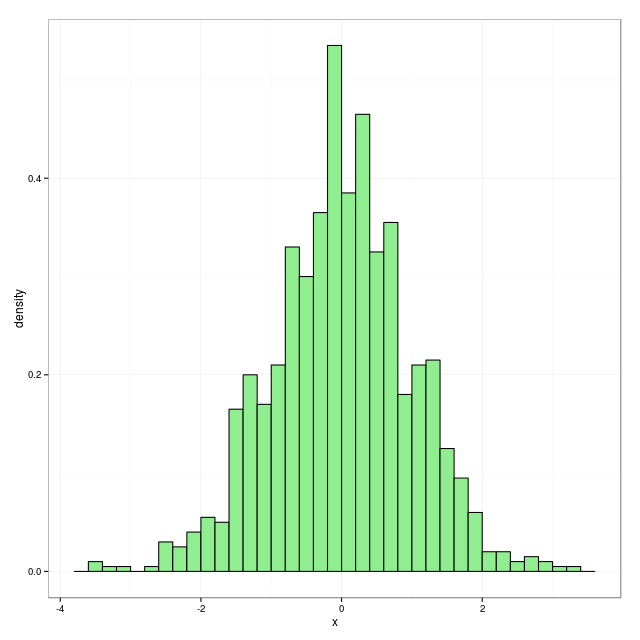
\includegraphics[width=0.5\linewidth]{pics/ris1}
	\caption{Связанная система координат квадрокоптера
	}
	\label{fig:ris1} % эта метка позволяет ссылаться на рисунок в тексте
\end{figure}
В качестве первого режима БПЛА \(U_{1}\) рассмотрим движение вдоль оси OZ, принадлежащей ССК. Данное движение обеспечивается одновременным увеличением скоростей винтов на одинаковое значение угловой скорости \(\Delta a\). Полученное при этом движение (рис. ~\ref{fig:ris1}) характеризуется взлетом или посадкой квадрокоптера (при нулевых значениях тангажа и крена) и описывается следующим выражением:
\begin{equation}
 U_{1}=b(\Omega_{1}^2+\Omega_{2}^2+\Omega_{3}^2+\Omega_{4}^2)
\end{equation}
где b – аэродинамическая составляющая тяги винта.
В качестве второго режима движения БПЛА \(U_{2}\) необходимо взять поворот вокруг оси OX, принадлежащей ССК. Данное движение достигается путем увеличения/уменьшения на величину \(\Delta a\) значения \(\Omega_{4}\) левого винта и уменьшением/увеличением на величину \(\Delta b\) значения \(\Omega_{1}\)
правого. Полученное при этом движение характеризуется изменением угла крена \(\phi\) (рис. ~\ref{fig:ris2}) и описывается следующим выражением:
\begin{equation}
U_{2}=lb(-\Omega_{2}^2-\Omega_{4}^2)
\end{equation}
где l – расстояние между центром квадрокоптера и центром винта.
% ~\ref{fig:ris2}
\begin{figure}[H]
	\centering
	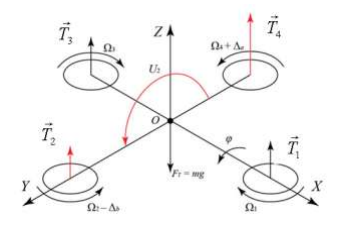
\includegraphics[width=0.5\linewidth]{pics/ris2}
	\caption{Вращение квадрокоптера вокруг оси OX
	}
	\label{fig:ris2} % эта метка позволяет ссылаться на рисунок в тексте
\end{figure}
В качестве третьего режима движения \(U_{3}\) необходимо взять поворот БПЛА вокруг оси OY , принадлежащей ССК. Данное движение достигается путем уменьшения/увеличения на величину \(\Delta a\) значения \(\Omega_{1}\) фронтального винта и увеличения/уменьшения на величину \(\Delta b\) значения \(\Omega_{3}\) заднего. Полученное при этом движение характеризуется изменением угла тангажа \(\theta\) (рис. ~\ref{fig:ris2}, а) и описывается следующим выражением:
\begin{equation}
U_{3}=lb(-\Omega_{1}^2-\Omega_{3}^2)
\end{equation}
% ~\ref{fig:ris3}
\begin{figure}[H]
	\centering
	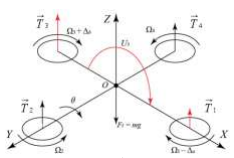
\includegraphics[width=0.5\linewidth]{pics/ris3}
	\caption{Вращение вокруг оси OY
	}
	\label{fig:ris3} % эта метка позволяет ссылаться на рисунок в тексте
\end{figure}
% ~\ref{fig:ris4}
\begin{figure}[H]
	\centering
	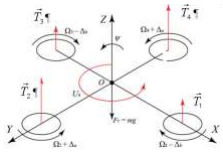
\includegraphics[width=0.5\linewidth]{pics/ris4}
	\caption{Вращение вокруг оси OZ
	}
	\label{fig:ris4} % эта метка позволяет ссылаться на рисунок в тексте
\end{figure}
Рис. 3 – Режимы движения квадрокоптера
